%TODO cite http://blog.gdeltproject.org/gdelt-2-0-our-global-world-in-realtime/
Recent GDELT updates provide feeds with 15-minute resolution, but historical feeds offered only daily resolution. We decided for simplicity to analyze daily changes in price, taking a full day's worth of news data into account. This was most in line with testing our hypothesis, that an aggregation of topic clusters in a day's news is predictive of commodity pricing.

Our data pipeline was designed to provide day-wise parallelism over our data set in order to enable fast testing of new feature extraction methods. The raw data, as well as intermediate data, is stored in TSV ASCII format.

\subsection{Model}

Every news event in GDELT is stored as a row in a file for that day's report. Every set of rows may undergo a series of transformations. First, in the \textbf{preprocessing} stage, we extract relevant topic- and importance- related columns. Next, in the \textbf{expansion} stage, we project each row to a purely real space, where we use a one-hot encoding for categorical values. Finally, in the \textbf{summary} stage, this purely numeric representation of each event in a set is summarized by a static clustering classification.

The day summaries are then conglomerated in a time series $\{\textbf{d}_i\}$. For a time series of a commodity's price, $\{p_i\}$, we have the corresponding sequence of binary labels indicating whether price has increased the next day, $y_i=1_{p_{i+1}>p_i}$.

Thus, our model assumes that:
\begin{enumerate}
\item The static clustering of news topics is accurate for the future.
\item $\mathbb{P}(p_{i+1}>p_i)$ may be determined by a regression over summaries $\textbf{d}_i$. 
\end{enumerate}

Both of these are strong assumptions. The first may be weakened by adapting a dynamic clustering model, such as an infinite Gaussian Mixture Model or an HDP. The second requires $\textbf{d}_i$ to be both contain a sufficient amount of information to predict price behavior, which is a matter of appropriate feature extraction, and the assumption that we do not lose too much predictive power in summarizing a day by aggregating over the clusters to which its news events belonged to.

\subsubsection{Vector Autoregressive}
VAR models are some of the most flexible and easy to use models for multivariate time series. They have proven to be especially useful for describing the dynamic behavior of economic and financial time series and for forecasting \cite{tsay, VAR}. \\
Let $Y_t = (y_1, y_2,...,y_nt)'$ denote an $(n \times 1)$ vector of time series variables. The basic p-lag vector autoregressive model (VAR(p)) has the form:
$$\bf{Y}_t=\bf{c}+\bf{\Pi}_1\bf{Y}_{t-1}+\bf{\Pi}_2\bf{Y}_{t-2}+\cdots+\bf{\Pi}_p\bf{Y}_{t-p}+\epsilon_t,$$ $$t=1\ldots T$$
where $\Pi_i$ are $(n \times n)$ matrix and $\epsilon_t$ is an $(n \times 1)$ unobservable zero mean noise vector process.

\subsubsection{L1 Linear model}

TODO(Ghassen)

TODO(Ghassen): Why we don't use Regimes with Markov-Switching and Impulse Response, why we dont use binary
%\subsubsection{Regimes and Markov-Switching}
%Recently, there has been work on Markov-Switching Vector Autoregressive Models (MSVAR) \cite{tsay}. In a Markov Switching Model the observed change in a variable between period t and t+1 is assumed to be a random draw from a distribution. Which distribution is appropriate depends  on an unobserved state variable $s_t$. When $s_t=1$, the observed change $y_t$ is drawn from $N(\mu_1,\sigma_1^2)$ and when $s_t=2$, the observed change $y_t$ is draw from $N(\mu_2,\sigma_2^2)$.
%The state variable is then assumed to evolve according to a Markov Chain such that the probability of being in state %1 at time t given that state 1 obtained at time t-1 equals $p_{11}$. Accordingly, we can build a transition matrix. There has been a decent amount of work that assumes the existence of 2 latent states (bullish vs. bearish market states) \cite{OIL}. MSVAR has also been used for high-frequency forecasts of foreign exchange markets \cite{MSVAR}.
%\subsubsection{Impulse Response}
%Since the contribution of Sims \cite{SIMS} the interaction between variables and disturbances in VAR models has been best described and interpreted by impulse response functions.
%An impulse response is when a shock is assigned to one variable of the system and where the propagation of this shock on all the variables of the system s studied over time.
%Impulse response functions are used to describe how the economy reacts over time to exogenous impulses, which economists usually call shocks. Impulse response functions describe the reaction of endogenous macroeconomic variables at the time of the shock and over subsequent points in time.
%The standard method to identify such shocks is through recursive identification where we impose a certain ordering to the variables, hence assuming that all contemporaneous interactions among variables are recursive. This corresponds to a B model allowing for instantaneous effects of the shocks on the variables which can be written as follows:
%$$y_t=A^{(0)}_{s_t}+\sum_{i=1}^p A^{(i)}_{s_t}y_{t-i}+B_{s_t}\epsilon_t$$
%Identifying the exact dates and the impact of these impulse responses can allow to better characterize big shifts in the markets that might (e.g. recessions) \cite{SIMS}.
\subsubsection{General Approach to Exogenous Factors}
There has been a lot of work on integrating exogenous factors (factors that are not caused by the financial data and are usual external to the financial systems/markets). VAR is, consequently, extended to accommodate a matrix of external events as follows \cite{VARX}: 
$$\bf{Y}_t=\bf{c}+\bf{\Pi}_1\bf{Y}_{t-1}+\bf{\Pi}_2\bf{Y}_{t-2}+\cdots+\bf{\Pi}_p\bf{Y}_{t-p}+\bf{\Phi D}_t+\bf{GX}_t+\epsilon_t$$
where $D_t$ represents an $(l \times l)$ matrix of deterministic components, $X_t$ represents an $(m \times 1)$ matrix of exogenous variable and $\Phi$ and $G$ are parameter matrices.
$\bf{y}_t=A^{-1}A^*_1\bf{y}_{t-1}+\ldots+A^{-1}A^*_p\bf{y}_{t-p}+A^{-1}A^*_1B\epsilon_t$

\subsubsection{ARIMA}
ARIMA stands for Auto-Regressive Integrated Moving Average. ARIMA models are, in theory, the most general class of models for forecasting a time series which can be made to be “stationary” by taking the difference (if necessary), perhaps in conjunction with nonlinear transformations such as logging or deflating (if necessary). A random variable that is a time series is stationary if its statistical properties are all constant over time.  A stationary series has no trend, its variations around its mean have a constant amplitude, and it wiggles in a consistent fashion, i.e., its short-term random time patterns always look the same in a statistical sense. The latter condition means that its auto-correlations (correlations with its own prior deviations from the mean) remain constant over time, or equivalently, that its power spectrum remains constant over time.  A random variable of this form can be viewed (as usual) as a combination of signal and noise, and the signal (if one is apparent) could be a pattern of fast or slow mean reversion, or sinusoidal oscillation, or rapid alternation in sign, and it could also have a seasonal component.  An ARIMA model can be viewed as a “filter” that tries to separate the signal from the noise, and the signal is then extrapolated into the future to obtain forecasts. Several works have built and tested Autoregressive Integrated Moving Average (ARIMA) models to forecast various econometric time series. For example, \cite{Vol} used ARIMA for realized volatility forecasting.

\subsection{Execution}

Our current implementation uses $K$-means for clustering and logistic regression for classification. We trained, validated, and sampled from the days between 2013-04-01 and 2015-07-31. Recent days were used for testing.

For our random sample, we sampled an equal number of events from each day. Even though days have variable numbers of events (and the number of reported events reduces as we go back in time), we chose this policy because the increase in news over recent years is not a property of more events occurring, but rather an increase in reporting, which should not affect the distribution of events among their hypothetical clusters of topics.

The random sample undergoes the same preprocessing and expansion pipeline as described below for the day summaries to be used in the regression, but its output is fed into a clustering model, that is then used in the main pipeline. We are forced to use a sample for tractability.

Raw data starts with 58 columns. Each day typically has 100K rows. Total size of the set is about 60GB. %TODO precise mean and stddev.

\begin{figure}[ht]
\vskip 0.2in
\begin{center}
\centerline{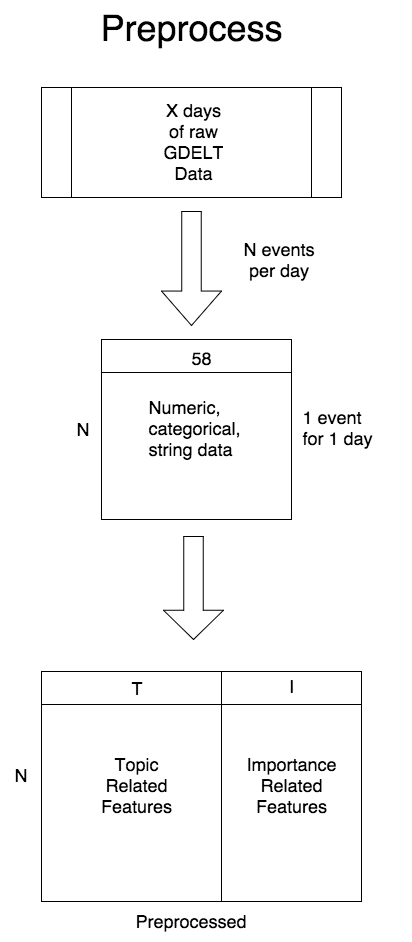
\includegraphics[scale=0.15]{images/preprocess_vertical.png}}
\caption{Preprocessing stage}
\end{center}
\vskip -0.2in
\label{fig:preprocess}
\end{figure}

After preprocessing, we are left with $T=12$ topic-related columns and $I=9$ importance columns, where the topic columns are in a compressed format, with categorical variables represented as integers and strings still as strings (though now sanitized and with stop words removed).

\begin{figure}[ht]
\vskip 0.2in
\begin{center}
\centerline{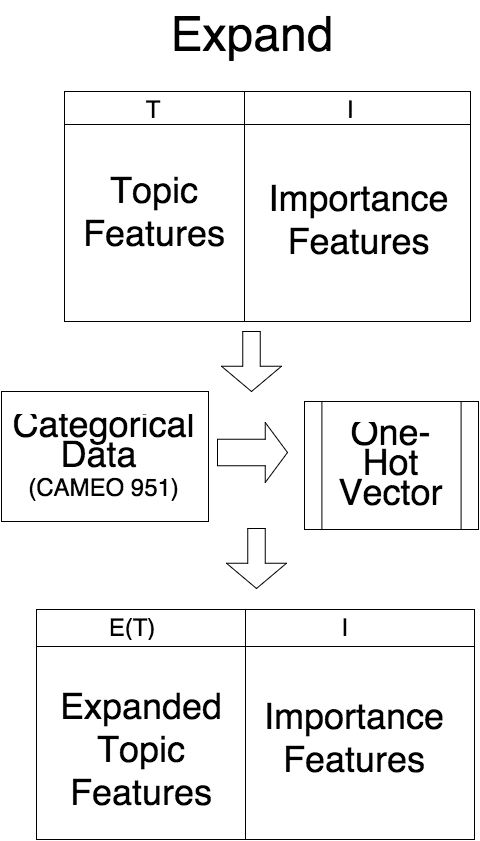
\includegraphics[scale=0.15]{images/expand_vertical.png}}
\caption{Expansion stage}
\end{center}
\vskip -0.2in
\label{fig:exapand}
\end{figure}

Expansion uses one-hot encoding on categorical features, such as the CAMEO code for the event.

%TODO mention here that we do sample-mean and sample-std-dev-based scaling, once we actually do that

\begin{figure}[ht]
\vskip 0.2in
\begin{center}
\centerline{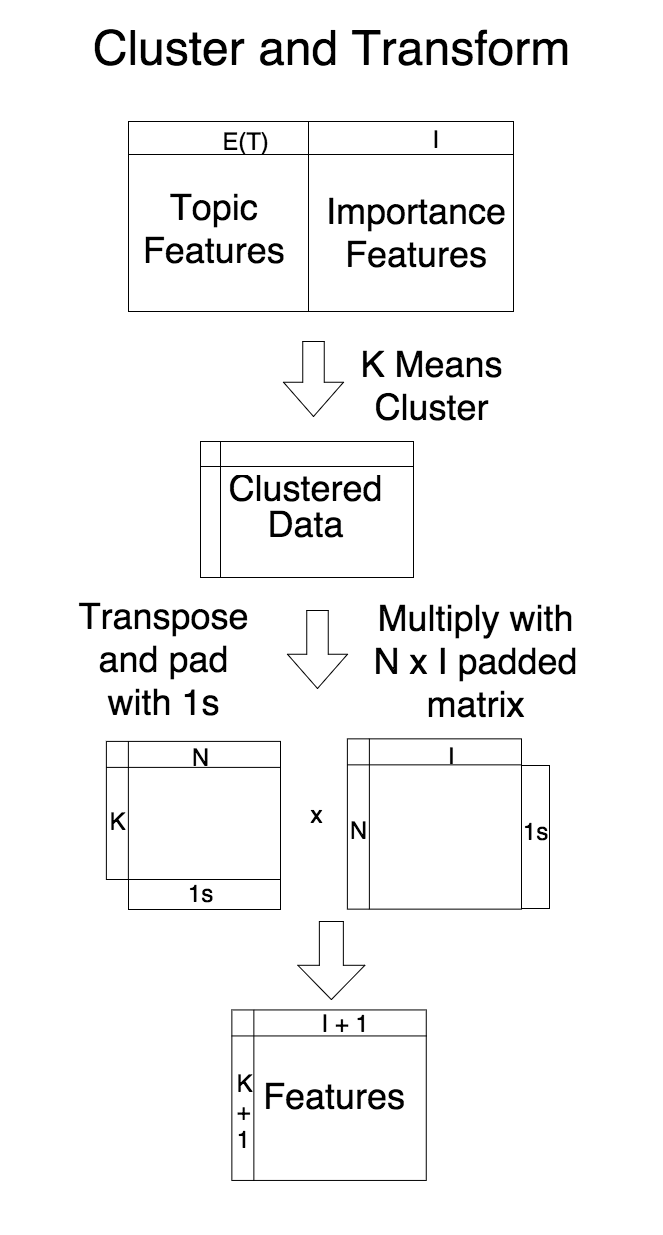
\includegraphics[scale=0.15]{images/cluster_and_transform_vertical.png}}
\caption{Summary stage}
\end{center}
\vskip -0.2in
\label{fig:summarization}
\end{figure}

The matrix multiply above conveniently extracts the sum of importance-weighted events belonging to certain topics. Note that this model is extensible to a mixture model, where each event's contribution to a topic's importance for that day is weighed by the probability of belonging to that topic's class. Furthermore, the aggregation creates a uniform description of every day, a flattened vector of dimension dependent on the cluster count.

These daily summaries were then enriched with historical pricing data before being fed into the linear model. The pricing data added was the 5, 10, and 30 day rolling average of the commodity price. %TODO hyperparam selection of rolling mean.
